\section{Opis problemu}
\label{sec:problem}

W rozdziale opisano dwa rozwiązywane zadania, sposób oceny ich rozwiązań, dostarczone zbiory danych oraz zakres badań wymagany w projekcie.

\subsection{Regresja i klasyfikacja}
\label{sec:problem-tasks}

Oba zadania należą do uczenia nadzorowanego (ang. \textit{supervised learning}). Dany jest zbiór uczący $\{(\mathbf{x}_i, y_i)\}_{i=1}^{n}$ par wejście-odpowiedź, na podstawie którego dobierane są parametry modelu. Celem nie jest jednak odtworzenie odpowiedzi ze zbioru uczącego, lecz poprawne przewidywanie dla nowych wejść. Dlatego jakość modelu ocenia się na osobnym zbiorze testowym, który nie jest używany w trakcie uczenia \cite{goodfellow2016}.

W zadaniu regresji wejściem jest liczba rzeczywista $x \in \mathbb{R}$, a odpowiedzią wartość $y \in \mathbb{R}$ pewnej nieznanej funkcji $f \colon \mathbb{R} \to \mathbb{R}$. Model zwraca przybliżenie $\yhat_i$ wartości $y_i$. Miarą jakości jest błąd średniokwadratowy (ang. \textit{mean squared error}, MSE) liczony na $m$ próbkach zbioru testowego w oryginalnej skali odpowiedzi:
\begin{equation}
    \mathrm{MSE} = \frac{1}{m} \sum_{i=1}^{m} \left( \yhat_i - y_i \right)^2 .
    \label{eq:mse}
\end{equation}

W zadaniu klasyfikacji wejściem jest wektor $\mathbf{x} \in \mathbb{R}^2$, a odpowiedzią numer klasy $y \in \{1, \dots, K\}$. Model zwraca rozkład prawdopodobieństwa na $K$ klasach, a decyzją $\yhat_i$ jest klasa o największym prawdopodobieństwie. Miarą jakości jest dokładność (ang. \textit{accuracy}), czyli odsetek poprawnie sklasyfikowanych próbek zbioru testowego:
\begin{equation}
    \mathrm{ACC} = \frac{1}{m} \sum_{i=1}^{m} \mathbf{1}\left[ \yhat_i = y_i \right] ,
    \label{eq:accuracy}
\end{equation}
gdzie $\mathbf{1}[\cdot]$ przyjmuje wartość $1$, gdy warunek jest spełniony, i $0$ w przeciwnym razie. Jeśli rozkłady klas nachodzą na siebie, w części przestrzeni wejść ta sama wartość $\mathbf{x}$ może należeć do różnych klas. Nawet optymalny klasyfikator, zwany klasyfikatorem Bayesa, myli się wtedy na części próbek, więc dokładność \qty{100}{\percent} jest nieosiągalna \cite{bishop2006}.

Miary \eqref{eq:mse} i \eqref{eq:accuracy} służą do oceny i porównywania modeli. Wielkość minimalizowana w trakcie uczenia, czyli funkcja straty, nie musi być z nimi tożsama. Funkcje straty opisano w podrozdziale~\ref{sec:mlp-losses}.

\subsection{Zbiory danych}
\label{sec:problem-datasets}

Do badań dostarczono cztery zbiory: dwa do klasyfikacji (\texttt{simple}, \texttt{three\_gauss}) i dwa do regresji (\texttt{activation}, \texttt{cube}). Każdy występuje w czterech licznościach zbioru uczącego, a każdej liczności towarzyszy plik testowy. Liczności zestawiono w Tabeli~\ref{tab:datasets}.

\begin{table}[H]
    \centering
    \caption{Dostarczone zbiory danych. Liczności podano jako liczbę próbek w pliku. W~\texttt{three\_gauss} każda klasa ma jedną trzecią próbek.}
    \label{tab:datasets}
    \begin{tabular}{llcll}
        \toprule
        Zbiór & Zadanie & Liczba klas & Liczności zbioru uczącego & Zbiór testowy \\
        \midrule
        \texttt{simple} & klasyfikacja & 2 & \numlist{100;500;1000;10000} & tej samej liczności \\
        \texttt{three\_gauss} & klasyfikacja & 3 & \numlist{300;1500;3000;30000} & tej samej liczności \\
        \texttt{activation} & regresja & --- & \numlist{100;500;1000;10000} & \num{1201} punktów \\
        \texttt{cube} & regresja & --- & \numlist{100;500;1000;10000} & \num{1201} punktów \\
        \bottomrule
    \end{tabular}
\end{table}

Zbiory klasyfikacji pokazano na Rysunku~\ref{fig:datasets-classification}. W zbiorze \texttt{simple} punkty wypełniają kwadrat $[-1, 1]^2$, a dwie klasy są rozdzielone prostą biegnącą wzdłuż przekątnej. Pojedyncze punkty leżą po niewłaściwej stronie tej prostej. Zbiór \texttt{three\_gauss} składa się z trzech równolicznych skupisk o różnych kształtach i rozrzutach, które częściowo na siebie nachodzą. W obszarze nakładania się skupisk przynależność punktu do klasy jest niejednoznaczna.

\begin{figure}[H]
    \centering
    \begin{subfigure}[b]{0.49\textwidth}
        \centering
        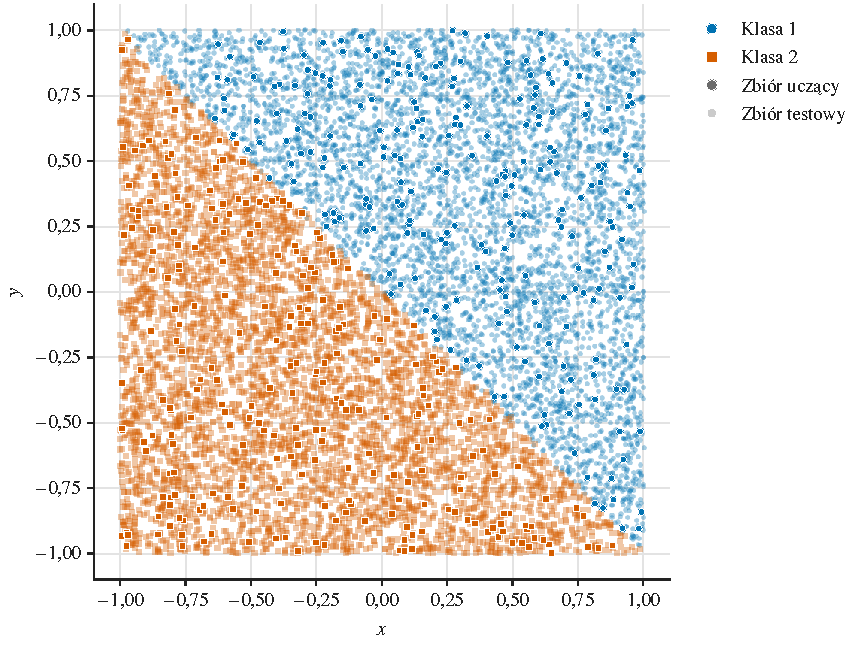
\includegraphics[width=\textwidth]{classification/showcase-simple/plots/dataset.pdf}
        \caption{\texttt{simple}}
    \end{subfigure}
    \hfill
    \begin{subfigure}[b]{0.49\textwidth}
        \centering
        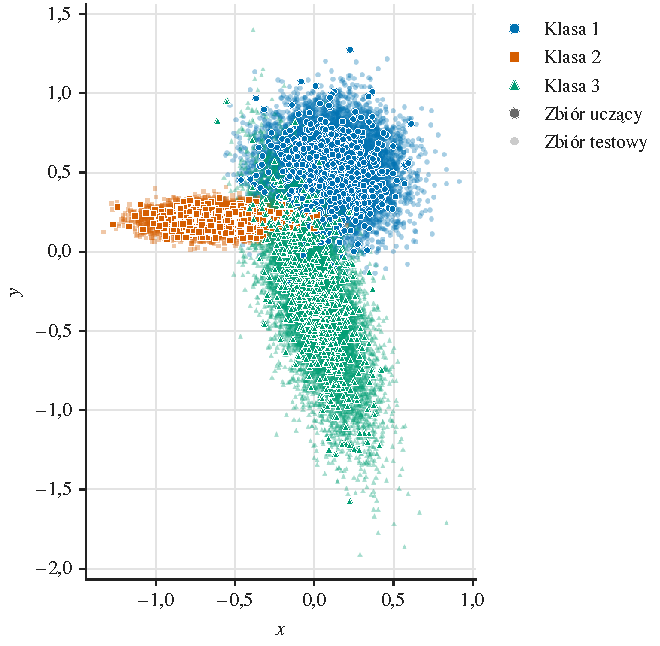
\includegraphics[width=\textwidth]{classification/showcase-three-gauss/plots/dataset.pdf}
        \caption{\texttt{three\_gauss}}
    \end{subfigure}
    \caption{Zbiory klasyfikacji: zbiór uczący o liczności \num{500} na rysunku~(a) i \num{1500} ($\num{500}$ na klasę) na rysunku~(b) oraz zbiór testowy o liczności \num{10000} na rysunku~(a) i \num{30000} na rysunku~(b).}
    \label{fig:datasets-classification}
\end{figure}

Zbiory regresji pokazano na Rysunku~\ref{fig:datasets-regression}. Funkcja w zbiorze \texttt{activation} jest monotoniczna i nasyca się na obu krańcach dziedziny, przyjmując kształt litery S. Funkcja w zbiorze \texttt{cube} ma przebieg krzywej sześciennej: między dwoma łagodnymi zagięciami jest prawie płaska, a na krańcach szybko rośnie co do wartości bezwzględnej. W obu zbiorach odpowiedzi są rzędu setek, a punkty uczące leżą blisko krzywej wyznaczonej przez zbiór testowy.

\begin{figure}[H]
    \centering
    \begin{subfigure}[b]{0.49\textwidth}
        \centering
        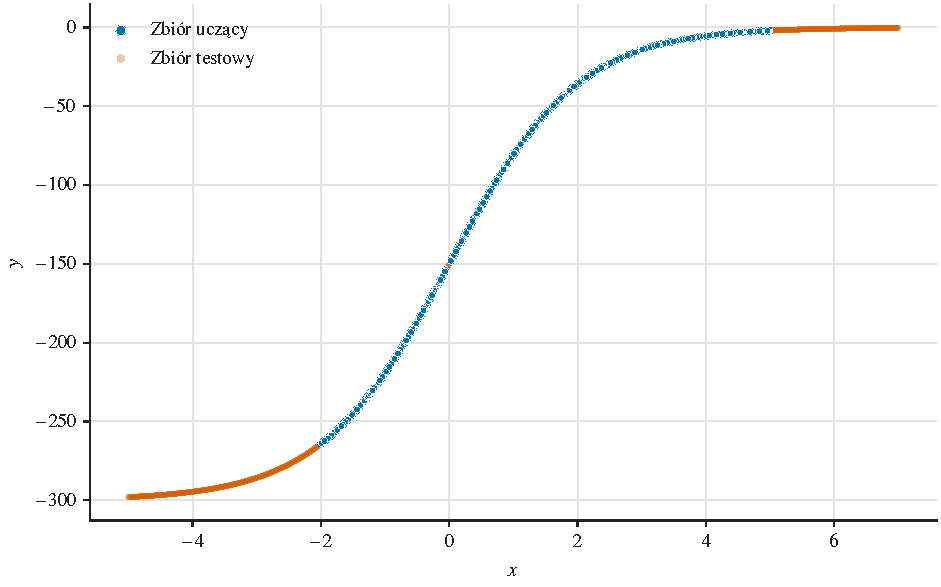
\includegraphics[width=\textwidth]{regression/showcase-activation/plots/dataset.pdf}
        \caption{\texttt{activation}}
    \end{subfigure}
    \hfill
    \begin{subfigure}[b]{0.49\textwidth}
        \centering
        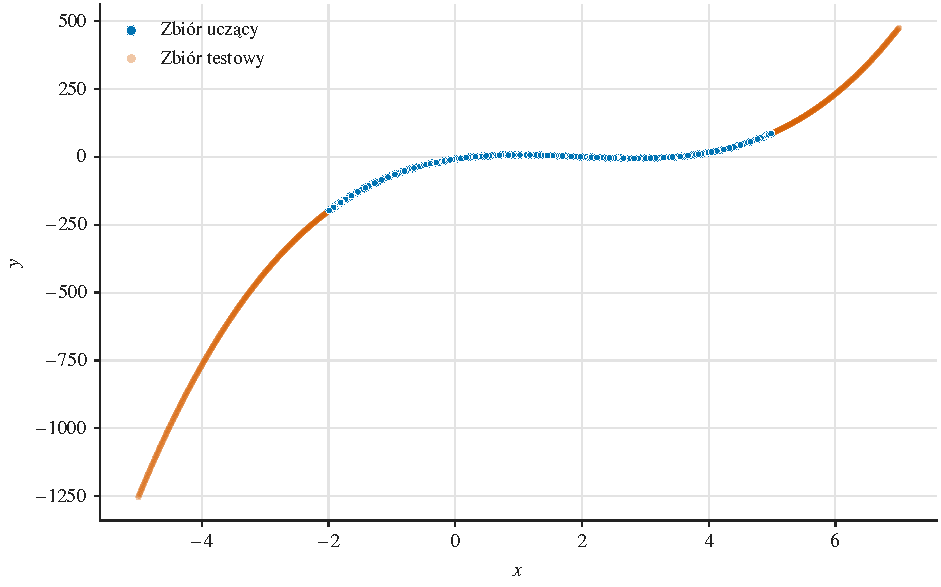
\includegraphics[width=\textwidth]{regression/showcase-cube/plots/dataset.pdf}
        \caption{\texttt{cube}}
    \end{subfigure}
    \caption{Zbiory regresji: zbiór uczący o liczności \num{500} i zbiór testowy o liczności \num{1201}.}
    \label{fig:datasets-regression}
\end{figure}

Zbiór testowy regresji jest jeden dla wszystkich liczności: \num{1201} punktów rozmieszczonych co \num{0.01} w przedziale $x \in [-5, 7]$. Wejścia zbiorów uczących leżą natomiast w przybliżeniu w przedziale $[-2, 5]$. Na części zbioru testowego model musi więc przewidywać wartości poza zakresem danych, na których był uczony, czyli ekstrapolować. Konsekwencje tego dla oceny modeli omówiono w podrozdziale~\ref{sec:methodology-metrics} i rozdziale~\ref{sec:regression}.

\subsection{Zakres badań}
\label{sec:problem-scope}

Zadanie projektowe wymaga implementacji perceptronu wielowarstwowego uczonego algorytmem propagacji wstecznej błędu z metodą stochastycznego spadku wzdłuż gradientu (ang. \textit{stochastic gradient descent}, SGD) lub jej wariantem, bez użycia bibliotek implementujących sieci neuronowe. Implementacja ma umożliwiać powtarzalne uczenie z zadanym ziarnem generatora liczb losowych oraz łatwą konfigurację liczby warstw, liczby neuronów w warstwach i obecności biasów. Wymagane są wizualizacje zbioru uczącego i wyników klasyfikacji oraz regresji, błędu w kolejnych iteracjach uczenia oraz wartości wag w kolejnych iteracjach.

Na dostarczonych zbiorach należy zbadać wpływ trzech czynników na skuteczność sieci:
\begin{itemize}
    \item funkcji aktywacji w warstwach ukrytych: funkcji sigmoidalnej i co najmniej dwóch innych, przy aktywacji wyjściowej dobranej do rodzaju zadania,
    \item liczby warstw ukrytych, od $0$ do $4$, oraz liczby neuronów w nich,
    \item funkcji straty: dwóch dla klasyfikacji i dwóch dla regresji.
\end{itemize}

Wynik uczenia zależy od losowej inicjalizacji wag i kolejności podawania próbek, więc pojedyncze uczenie nie wystarcza do porównania wariantów. Zadanie wymaga zaadresowania tego problemu, dlatego każdy wariant uczono dla wielu ziaren generatora.

Model sieci i algorytm uczenia opisano w rozdziale~\ref{sec:mlp}, a ich implementację w rozdziale~\ref{sec:implementation}. Wymagane wizualizacje przedstawiono w rozdziale~\ref{sec:showcase}, a plan badań w rozdziale~\ref{sec:methodology}.
